\documentclass{article}
\usepackage{graphicx}
\graphicspath{{Figure/}}
\usepackage{amsmath}
\numberwithin{equation}{section} % Will include section number in equation number as X.Y
\usepackage[letterpaper, total={6.5in, 9in}]{geometry}
\bibliography{Bibliographie}
\renewcommand{\contentsname}{Table des matières} %Allow to change "Content" to "Table des matières"

% Document metadata and general information
\title{Travail noté sur les vues et l'indexation}
\author{Pascal Perron-Abran}
\date{\today}
\bibliographystyle{ieeetr}

%Start of the document
\begin{document}
\maketitle
\begin{abstract}
    Ce travail a été préparé dans le cadre du cours INF6408 - Informatique de l'analyse multidimensionnelle. L'objectif est de développer la compréhension de l'indexation, principalement les index bitmap et la representation ORDPATH pour un fichier XML. Comme objectif individuel, nous avons aussi décidé de travailler nos aptitudes \LaTeX{} et Github.
\end{abstract}

\newpage
\tableofcontents

\newpage


\section{Question 1}
Pour la première colonne, nous devons donc créer un bitmap par mois, pour un total de 12 bitmaps. Dans la deuxième colonne, 16 bitmaps et, pour la troisième colonne, dix bitmaps.

Dans ce scénario, 38 bitmaps seront créés.

\section{Question 2}
La représentation ORDPATH, est une représentation hiérarchique des étiquettes XML. Lors de la création de cette représentation, seuls les entiers impairs seront utilisés afin de permettre l'insertions de nouveaux éléments lorsque nécessaire \cite{ACM}
    \begin{figure}[!ht]
        \centering
        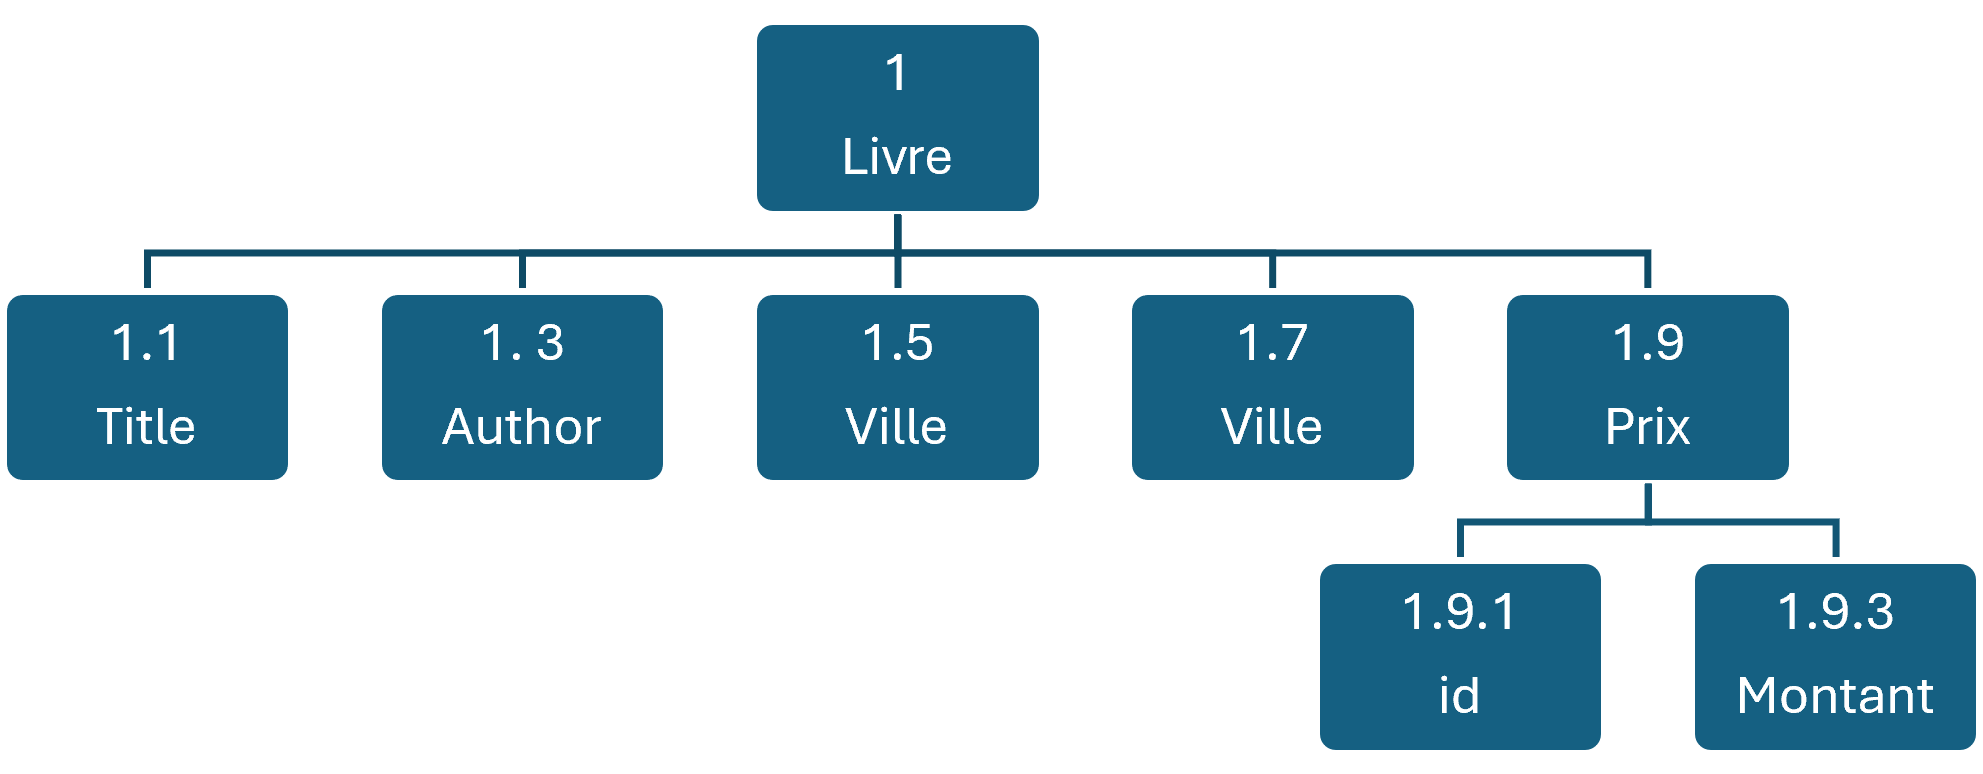
\includegraphics[width=0.75\textwidth]{hierarchical}
        \caption{Représentation hiérarchique du fichier XML}
        \label{fig:hierarchy}
    \end{figure}

    \begin{table}[!ht]
        \begin{center}
            \begin{tabular}{|| c | c | c | c ||}
                \hline
                \textbf{ORDPATH} & \textbf{Nom} & \textbf{Type} & \textbf{Valeur} \\
                \hline
                \hline
                1   & book & Élément & S.O.\\
                1.1 & title & Élément & La vie est belle\\
                1.3 & author & Élément & Jean Égard\\
                1.5 & ville & Élément & Montréal\\
                1.7 & ville & Élément & Paris\\
                1.9 & prix & Élément & S.O.\\
                1.9.1 & id & Attribut & 14444\\
                1.9.3 & montant & Élément & 104.00\\
                \hline
            \end{tabular}
        \end{center}
        \caption{Representation ORDPATH d'un document XML}
        \label{table:ordpath}
    \end{table}
    
\section{Question 3}
Considérons que la base de données de la question 1 contienne \textit{n} enregistrements, est organisée en \textit{m = 3} colonnes et que chaque valeur est stockée dans un registre de taille \textit{s}. Si elle est organisée en \textit{rangée}, et que nous voulons faire une recherche sur \textit{k} colonne, tel que \textit{k $\leq$ 3}, nous pouvons utiliser l'équation \ref{eq:size_row} pour calculer la taille des données chargées \cite{Lee_2026}.

\begin{equation}
    D_{rang\acute{e}e} = n \cdot s \cdot m
    \label{eq:size_row}
\end{equation}


Si nous avons la même base de données orientée \textit{colonne} et que nous voulons faire la même requête sur \textit{k} colonnes, la taille des données chargées peut etre obtenue par l'équation \ref{eq:size_col} (ibid.). Il est intéressant de noter que, en combinant les équations \ref{eq:size_row} et \ref{eq:size_col}, nous trouvons que le ratio entre la taille des données chargées ne dépend que du ratio k/m (voir l'équation \ref{eq:ratio}).
\begin{equation}
    D_{colonne} = n \cdot s \cdot k
    \label{eq:size_col}
\end{equation}

\begin{equation}
    \frac{D_{colonne}}{D_{rang\acute{e}e}} = \frac{n \cdot s \cdot k}{n \cdot s \cdot m} = \frac{k}{m}
    \label{eq:ratio}
\end{equation}
Par conséquent, l'orientation \textit{colonne} nous permet de charger moins de données que l'orientation \textit{rangée}, tant que le nombre de colonne sur lesquelles nous faisons une requête est de $k \leq 2$ et, si $k=m$, les deux orientations auront la même performance.



De plus, nous pouvons optimiser les performances de l'orientation colonne en triant les données selon la colonne ayant le moins de valeurs possible (faible cardinalité). Dans notre cas, ce tri serait basé sur la colonne \textit{Province}. Nous pourrions ensuite procéder au codage par plage. En reprenant l'exemple de la question d'approfondissement \cite{Lemire_2026}, et considérant que la colonne \textit{Mois} a douze valeurs possibles, la colonne \textit{Année}, seize, et la colonne \textit{Province}, dix, notre pire scénario contiendrait 10 x 12 x 16 = 1 920 plages. 

\end{document}